\mySection{The Design of PyRollCall}
In this section, we present the use cases and the design and PyRollCall's architecture.
In the following context, a "user" refers to a "teacher" who wishes to perform roll calls
using this system, since the end user of PyRollCall is typically a teacher. In other words,
students are not the direct users of this system.
Figure~\ref{fig:use-case-diagram} shows the use case diagram of PyRollCall, whereas
Figure~\ref{fig:system-architecture} shows the system architecture of PyRollCall.

\subsection{Use Cases}
\vspace{0.5cm}

\setstretch{1.0}
\begin{itemize}
  \item Users can maintain the data of the courses and students they teach.
  \item Users can collect students' photos and generate their facial measurements.
  \item Users can start a roll call, recording students' attendace via FRT.
  \item Users can export the results of roll calls to files.
  \item Users should be able to keep their data the next time they use the system.
  \end{itemize}
\setstretch{\myContentLineSpacing}

\begin{figure}[!htb]
  \centering
  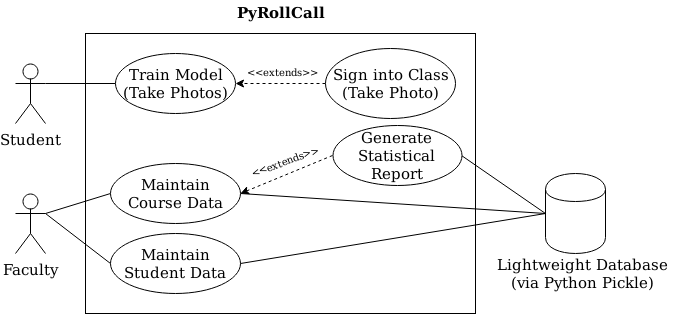
\includegraphics[width=\linewidth]{figures/use-case-diagram.png}
  \caption{Use Case Diagram}
  \label{fig:use-case-diagram}
\end{figure}

\subsection{System Architecture}
\begin{figure}[!htb]
  \centering
  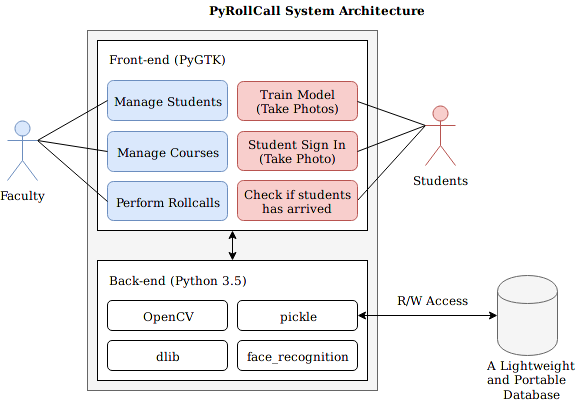
\includegraphics[width=\linewidth]{figures/system-architecture.png}
  \caption{System Architecture}
  \label{fig:system-architecture}
\end{figure}
